%
\documentclass{beamer}

% document encoding
% http://tex.stackexchange.com/questions/44694/fontenc-vs-inputenc
\usepackage[T1]{fontenc}
\usepackage[utf8]{inputenc}
\usepackage[english]{babel} %set language to english

\usepackage{logreq}
% needs to be high up to clear error
% (/usr/share/texlive/texmf-dist/tex/latex/biblatex/biblatex2.sty
% (/usr/share/texlive/texmf-dist/tex/latex/logreq/logreq.sty
% ! Undefined control sequence.
% l.163 \newrobustcmd
%                    *{\DeclareLogreqContainer}{\lrq@defparser\lrq@container}

\RequirePackage[l2tabu, orthodox]{nag}
\usepackage{verbatim}

%% fonts

%\usepackage{pxfonts}
%\usepackage[]{helvet}
%\usepackage{times}
%\renewcommand\rmdefault{phv}% helvet

%%------------------------------------------------
%% style
% Customize slide appearance
%\mode<presentation>
{
  \usetheme{Warsaw} %mtheme seems incompatible with tikz
  \setbeamercovered{transparent}
}
\setbeamertemplate{navigation symbols}{} % don't use navigation tools on slides
%\usepackage{kantlipsum}

%%------------------------------------------------
%% notes
%\usepackage{pgfpages}
%\setbeameroption{show notes on second screen=left}
%%------------------------------------------------


%%------------------------------------------------
%% packages
\usepackage{amsmath,amssymb,amsfonts}
\usepackage{tikz, graphicx}


%%% video packages
%\usepackage[absolute,overlay]{textpos} 
%\usepackage{graphicx}
%\usepackage{extrabeamercmds}    
\usepackage[loop,controls,buttonsize=0.24cm,buttonbg=0.8,autoplay]{animate}


%--------------------------
%% colors
%\usepackage{colortbl}
%\definecolor{Golden}{RGB}{184,134,11}
%\definecolor{tblcolorA}{rgb}{0.9 0.9 0.9} 
%\definecolor{tblcolorB}{rgb}{0.7 0.7 0.9} 
%\definecolor{colCONCLUSION}{rgb}{0.0 0.5 0.1 }
%--------------------------




% You can add any graphics to every slide by following command:
% \logo{
\includegraphics{logo.eps}}
% Uncomment this, if you want the table of contents before each subsection.
% However, to edit slides in TeXWord avoiding this feature is good idea.
% \AtBeginSubsection[]
% {
%   \begin{frame}<beamer>
%     \frametitle{Outline}
%     \tableofcontents[currentsection,currentsubsection]
%   \end{frame}
% }

% If you wish to uncover everything in a step-wise fashion, uncomment
% the following command: 
%\beamerdefaultoverlayspecification{<+->}




%%%%%%%%%%%%%%%%%%%%%%%%%%%%%%%%%5
%% BIBLIOGRAPHY SETTINGS
%%%%%%%%%%%%%%%%%%%%%%%%%%
%footnote citations
\usepackage[citestyle=numeric-comp,hyperref=true, sorting=none,autocite=superscript,backend=biber]{biblatex}
%%\def\bibfont{\footnotesize}
%\usepackage{hyperref}
%\usepackage[citestyle=numeric-comp,hyperref=true, sorting=none]{biblatex}
%\usepackage[citestyle=numeric-comp, sorting=none]{biblatex}
%% Define \citejournal
%% http://tex.stackexchange.com/questions/26682/how-to-create-a-citejournal-citebooktitle-cite-command-in-biblatex
\DeclareCiteCommand{\citejournal}
  {\usebibmacro{prenote}}
  {\usebibmacro{citeindex}%
    \usebibmacro{journal}}
  {\multicitedelim}
  {\usebibmacro{postnote}}

\DeclareCiteCommand{\citebooktitle}
  {\usebibmacro{prenote}}
  {\usebibmacro{citeindex}%
    \usebibmacro{booktitle}}
  {\multicitedelim}
  {\usebibmacro{postnote}}

\DeclareCiteCommand{\citeintitle}% Based on \citetitle from biblatex.def
  {\boolfalse{citetracker}%
   \boolfalse{pagetracker}%
   \usebibmacro{prenote}}
  {\ifciteindex
     {\indexfield{indextitle}}
     {}%
   \iffieldundef{journaltitle}
     {\iffieldundef{booktitle}
        {\iffieldundef{maintitle}
          {\printfield[citetitle]{labeltitle}}% Behave like \citetitle if no "main" title
          {\printtext[maintitle]{\printfield[titlecase]{maintitle}}}}
        {\printtext[booktitle]{\printfield[titlecase]{booktitle}}}}
     {\printtext[journaltitle]{\printfield[titlecase]{journaltitle}}}}
  {\multicitedelim}
  {\usebibmacro{postnote}}

%%----------------------------------------------------
%%Footnote
%%% provides \ctfoot{Liu1998}
%%% presently limited to up to four authors at once
%%% Note, for variable number of inputs use \ctfoott (2 inputs), \ctfoottt (3 inputs), etc
\newfont{\smallfont}{phvr at 5 pt}
\newfont{\tablefont}{phvr at 7 pt}
\newcommand{\cst}[1]{\textsuperscript{\cite{#1}}}
\newcommand{\cstt}[2]{\textsuperscript{\cite{#1,#2}}}
\newcommand{\csttt}[3]{\textsuperscript{\cite{#1,#2,#3}}}
\newcommand{\ctauthoryear}[1]{\citeauthor{#1} [\citeyear{#1}]}
\newcommand{\ctauthoryearsm}[1]{\smallfont \citeauthor{#1} [\citeyear{#1}]}
\newcommand{\ctfoota}[1]{\cite{#1} \citeauthor{#1} (\citeyear{#1}). \citeintitle{#1}}
\newcommand{\ctfoot}[1]{\let\thefootnote\relax\footnotetext{\smallfont \hskip-0.5em \ctfoota{#1}}}
\newcommand{\ctfoott}[2]{\let\thefootnote\relax\footnotetext{\smallfont \hskip-0.5em \ctfoota{#1}; \ctfoota{#2} }}
\newcommand{\ctfoottt}[3]{\let\thefootnote\relax\footnotetext{\smallfont \hskip-0.5em \ctfoota{#1}; \ctfoota{#2}; \ctfoota{#3} }}
\newcommand{\ctfootttt}[4]{\let\thefootnote\relax\footnotetext{\smallfont \hskip-0.5em \ctfoota{#1}; \ctfoota{#2}; \ctfoota{#3}; \ctfoota{#4} }}
\renewcommand{\footnotesize}{\fontsize{6}{8}\selectfont} 



% info
\author{Author Name}
\title{My Title}
%\subtitle[My subtitle\hspace{2em}\insertframenumber/\inserttotalframenumber]{}
\date{January 11, 2016} %leave out for today's date to be insterted
\institute{Department of Physics \\ University of Pennsylvania}
%==============================================================================



%%%%%%%%%%%%%%%%%%%%%%%%%%%%%%%%%%%%%%%%%%%%%%%%%%%%%%%%%
% file paths
%%%%%%%%%%%%%%%%%%%%%%%%%%%%%%%%%%%%%%%%%%%%%%%%%%%%%%%%%%%%
\usepackage{ifthen}
\newboolean{isLinux}
\setboolean{isLinux}{true} %true Linux; false Win
\ifthenelse{\boolean{isLinux}}{\graphicspath{{./},{../},{./apollo17/}}}{\graphicspath{{beamer/}}}
\ifthenelse{\boolean{isLinux}}{\bibliography{../library} }{\bibliography{C:/Users/username/Documents/library}}
%\graphicspath{{./},{../},{./apollo17/}}
%%%%%%%%%%%%%%%%%%%%%%%%%%%%%%%%%%%%%%%%%%%%%%%%%%%%%%%%%%%%%%%%%%%





%%%%%%%%%%%%%%
%tiz utils
\usepackage{tikzscale}
\usepackage{filecontents}   % to write tikz on the fly
%%%%%%%%%%%%%%%%%%%%%%%%%%%%%%%%%%%%%%%%%%%%%%%%%%%%%%%%%%%%%%%%%%
% mindmap tikz example
% source: http://www.texample.net/tikz/examples/servers/

\usepackage{dtklogos}

%\usepackage{tikz}
\usetikzlibrary{mindmap,shadows}
%\usepackage[hidelinks,pdfencoding=auto]{hyperref}
% Information boxes
\newcommand*{\info}[4][16.3]{%
  \node [ annotation, #3, scale=0.65, text width = #1em,
          inner sep = 2mm ] at (#2) {%
  \list{$\bullet$}{\topsep=0pt\itemsep=0pt\parsep=0pt
    \parskip=0pt\labelwidth=8pt\leftmargin=8pt
    \itemindent=0pt\labelsep=2pt}%
    #4
  \endlist
  };
}

\begin{filecontents*}{mindmap.tikz} 
  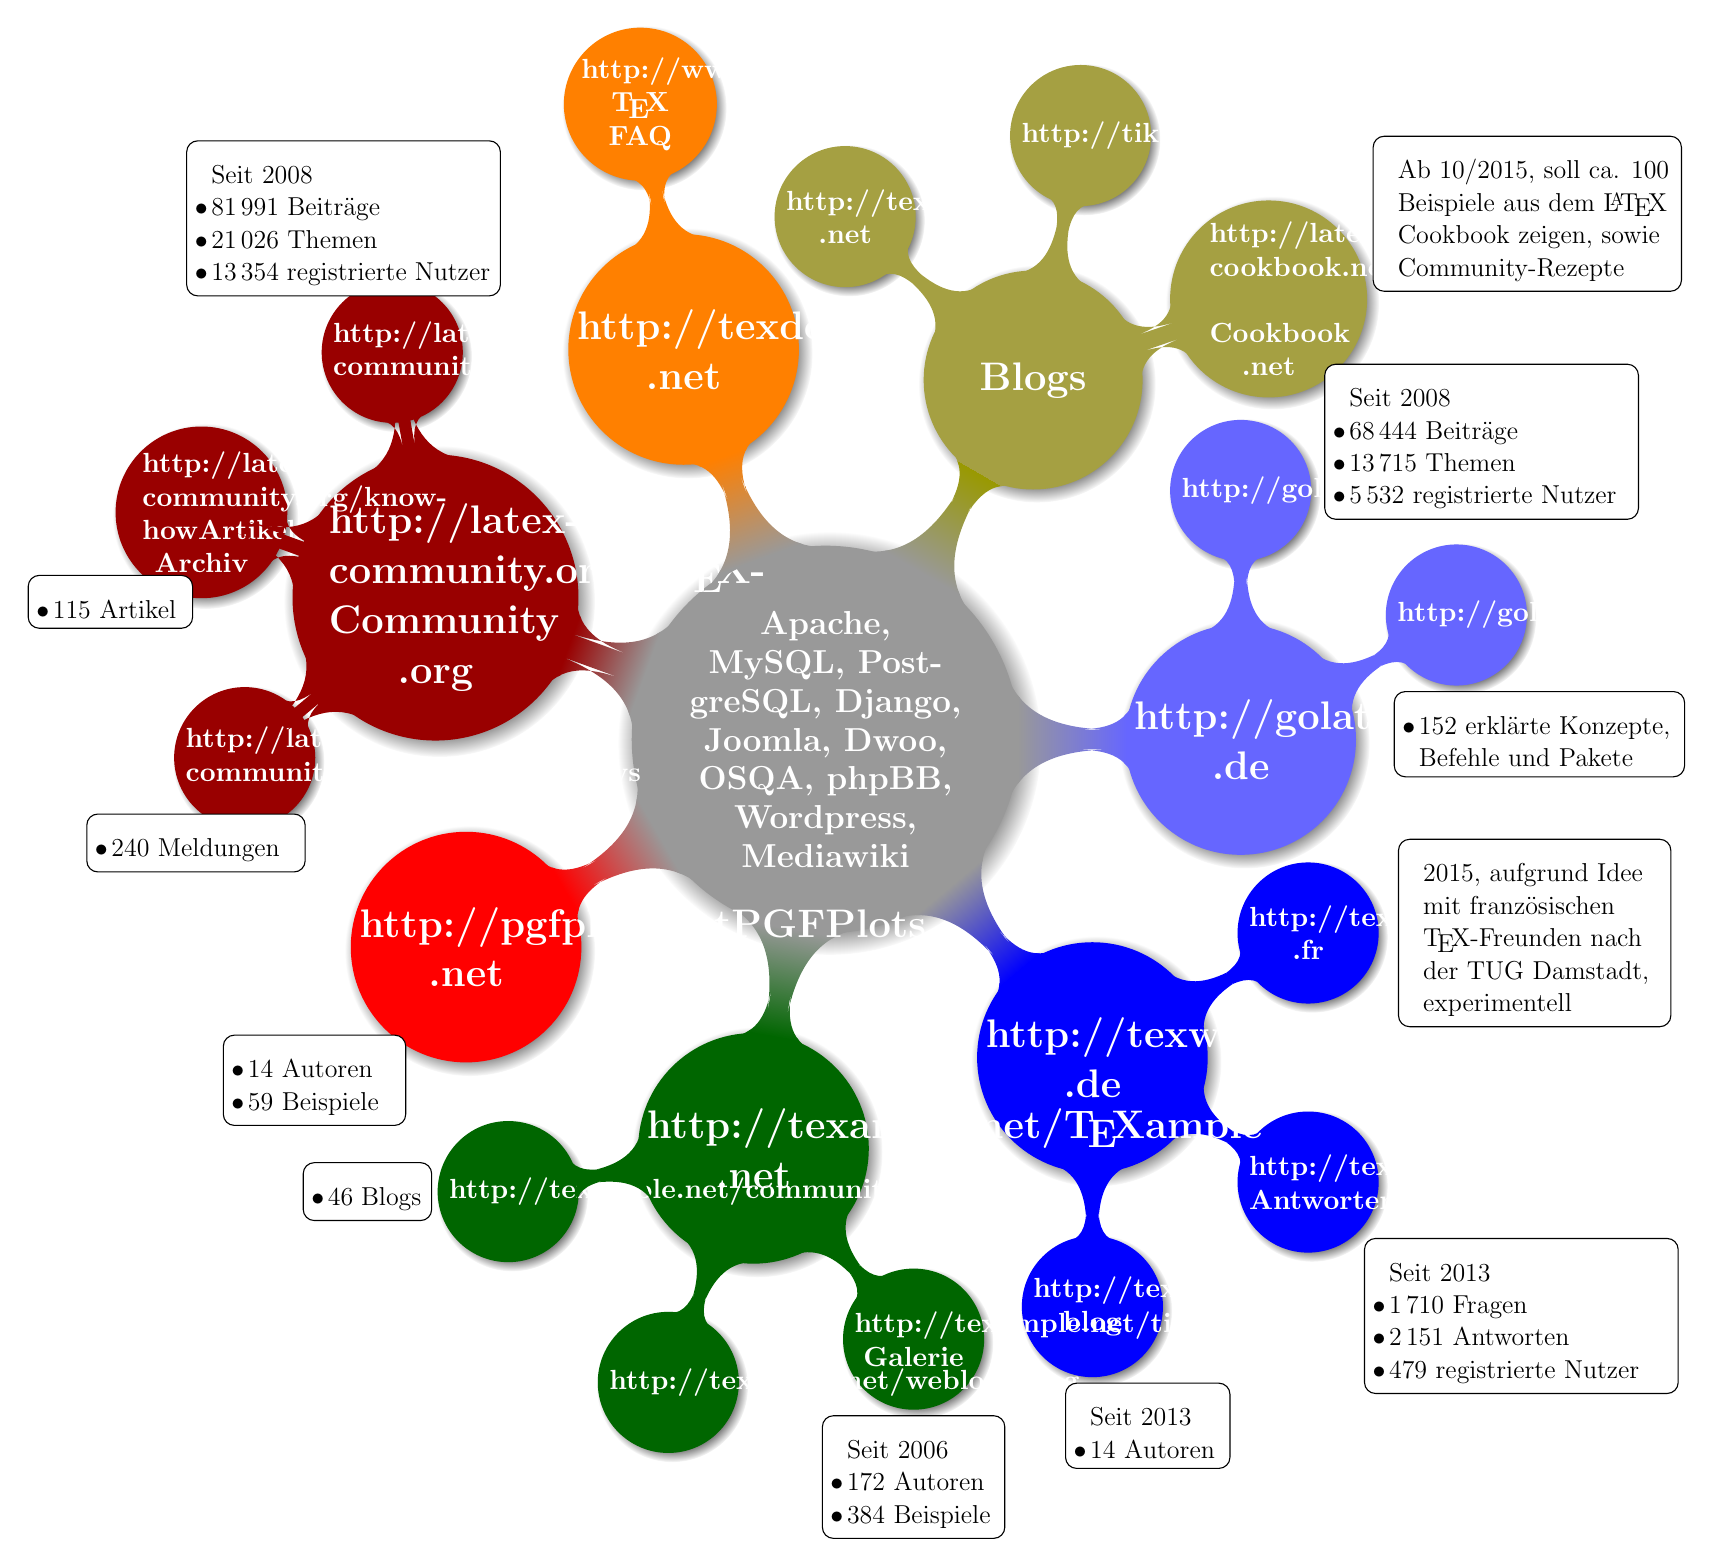
\begin{tikzpicture}[ every annotation/.style = {draw,
                     fill = white, font = \Large}]
  \path[mindmap,concept color=black!40,text=white,
    every node/.style={concept,circular drop shadow},
    root/.style    = {concept color=black!40,
      font=\large\bfseries,text width=10em},
    level 1 concept/.append style={font=\Large\bfseries,
      sibling angle=50,text width=7.7em,
    level distance=15em,inner sep=0pt},
    level 2 concept/.append style={font=\bfseries,level distance=9em},
  ]
  node[root] {Apache, MySQL, PostgreSQL, Django, Joomla,
    Dwoo, OSQA, phpBB, Wordpress, Mediawiki} [clockwise from=0]
    child[concept color=blue!60] {
      node {\href{http://golatex.de}{go\LaTeX\\.de}} [clockwise from=90]
        child { node (goForum) {\href{http://golatex.de/index.html}{Forum}} }
        child { node (goWiki) {\href{http://golatex.de/wiki/Hauptseite}{Wiki}} }
    }
    child[concept color=blue] {
      node[concept] {\href{http://texwelt.de}{\TeX welt\\.de}}
        [clockwise from=30]
      child { node[concept] (TeXnique)
        {\href{http://texnique.fr}{\TeX nique\\.fr}} }
      child { node[concept] (TeXweltQA)
        {\href{http://texwelt.de/wissen/}{Fragen~\& Antworten}} }
      child { node[concept] (TeXweltBlog)
        {\href{http://texwelt.de/blog/}{User blog} }}
    }
    child[concept color=green!40!black] {
      node[concept] {\href{http://texample.net/}{\TeX ample\\.net}}
        [clockwise from=310]
      child { node[concept] (TikZGalerie) 
        {\href{http://texample.net/tikz/examples/}{TikZ-Galerie}} }
      child { node[concept] (TeXampleBlog)
        {\href{http://texample.net/weblog/}{Blog}} }
      child { node[concept] (Planet)
        {\href{http://texample.net/community/}{Planet}} }
    }
    child[concept color=red] {
      node[concept] (PGFPlots) {\href{http://pgfplots.net}{PGFPlots\\.net}}
      [clockwise from=270]
    }
    child[concept color=red!60!black] {
      node[concept] {\href{http://latex-community.org/}{\LaTeX-Community\\.org}}
        [counterclockwise from=100]
      child { node[concept] (LaTeXForum)
        {\href{http://latex-community.org/forum/}{Forum}}}
      child { node[concept] (LaTeXArtikel)
        {\href{http://latex-community.org/know-how}{Artikel-Archiv}} }
      child { node[concept] (LaTeXNews)
        {\href{http://latex-community.org/home/news}{News}} }
    }
    child[concept color=orange] {
      node[concept] (TeXdoc)
        {\href{http://texdoc.net/}{\TeX doc\\.net}}
        [clockwise from=100]
        child { node[concept] {\href{http://www.tex.ac.uk}{UK \TeX \\FAQ}}
        }}
    child[concept color=yellow!60!black] {
      node[concept] (Blogs) {Blogs} [clockwise from=139]
      child { node[concept] {\href{http://texblog.net/}{\TeX blog\\.net}}}
      child { node[concept] {\href{http://tikz.de/}{TikZ.de}} }
      child { node[concept] (Cookbook)
        {\href{http://latex-cookbook.net/}{\LaTeX-\\Cookbook\\.net}} }
    };
    \info{goForum.north east}{above,anchor=west,xshift=1em}{%
      \item[] Seit 2008
      \item 68\,444 Beiträge
      \item 13\,715 Themen
      \item 5\,532 registrierte Nutzer
    }
    \info{LaTeXForum.north west}{above,anchor=south}{%
      \item[] Seit 2008
      \item 81\,991 Beiträge
      \item 21\,026 Themen
      \item 13\,354 registrierte Nutzer
    }
    \info[8]{LaTeXArtikel.west}{below,anchor=north east,xshift=3em,yshift=-2em}{%
      \item 115 Artikel
    }
    \info[11]{LaTeXNews.south west}{below,anchor=north}{%
      \item 240 Meldungen
    }
    \info[9]{TikZGalerie.south}{below,anchor=north}{%
      \item[] Seit 2006
      \item 172 Autoren
      \item 384 Beispiele
    }
    \info[15]{goWiki.south}{below,anchor=north,xshift=3em}{%
      \item 152 erklärte Konzepte, Befehle und Pakete
    }
    \info{TeXweltQA.south east}{above,anchor=north west}{%
      \item[] Seit 2013
      \item 1\,710 Fragen
      \item 2\,151 Antworten
      \item 479 registrierte Nutzer
    }
    \info[8]{TeXweltBlog.south}{below,anchor=north,xshift=2em}{%
      \item[] Seit 2013
      \item 14 Autoren
    }
    \info[9]{PGFPlots.south west}{anchor=north east,xshift=1em}{%
      \item 14 Autoren
      \item 59 Beispiele
    }
    \info[6]{Planet.west}{anchor=east}{%
      \item 46 Blogs
    }
    \info[14]{TeXnique.east}{anchor=west,xshift = 0.5em}{%
      \item[] 2015, aufgrund Idee mit französischen
              \TeX-Freunden nach der TUG Damstadt, experimentell
    }
    \info[16]{Cookbook.east}{anchor=south west}{%
      \item[] Ab 10/2015, soll ca. 100 Beispiele aus
              dem \LaTeX\ Cookbook zeigen, sowie
              Community-Rezepte
    }
\end{tikzpicture}
\end{filecontents*}




%%%%%%%%%%%%%%%%%%%%%%%%%%%%%%%%
%load files. 
% I notice improved stability doing this at the end of the preamble

%\usepackage{hyperref} % has to be after hypersetup
\usepackage{filecontents}

\input{abbreviations.bib}


% you can generate this file automatically. See the Makefile.
% \begin{filecontents}{\abbreviations.bib}
% %http://tex.stackexchange.com/questions/66549/short-titles-journal-abbreviations-etc-in-biblatex % a longer example
% % https://github.com/gvdgdo/biblatex-lncs/blob/master/lncs.bbx
% % 
% % % How to do abbreviations manually
% \DeclareSourcemap{%
%   \maps[datatype=bibtex]{
%     % Journal abbreviations
%     \map{
%       \step[fieldsource=journaltitle, match={Organometallics},
%       replace={Org}]%
%        \step[fieldsource=booktitle, match={Aristotle on Mind and the Senses},
%       replace={ AMS}]%
%        \step[fieldsource=booktitle, match={Aristotle on Mind and the Senses},
%       replace={ AMS}]%      
%     }
%   }
% }
% \end{filecontents}

%\addbibresource{mybib.bib}
\bibliography{mybib}

%%%%%%%%%%%%%%%%%%%%%%%%%%%%%%%%%%%%%%%%%%%%%%%%%%%%%%%%%%%%%%%%%%%%%%%%%%%%%%%
\begin{document}

%%%%%%%%%%%%%%%%%%%%%%%%%%%%%%%%%%%%%%%%%%%%%%%%%%%%%%%%%%%%%%%%%%%%%%%%%%%%%%%


%%%%%%%%%%%%%%%%%%%%%%%%%%%%%
%%% begin title page
%%%%%%%%%%%%%%%%%%%%%%%%
\addtocounter{framenumber}{-1}

% STYLING FOR TITLE SLIDE
%http://tex.stackexchange.com/questions/261004/help-with-size-of-an-image-for-a-book
\setbeamercolor{background canvas}{bg=violet}
\setbeamercolor{title}{fg=black} % title line color
\setbeamertemplate{background}{\tikz[overlay,remember picture]\node[opacity=0.4] at (current page.center){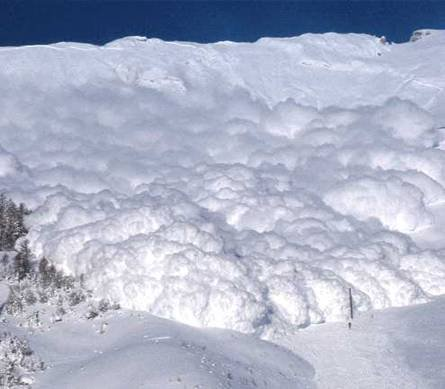
\includegraphics[width=\textwidth]{titlebackground.png}};}
%\setbeamertemplate{background}{\begin{tikzpicture}[overlay,remember picture]\node[opacity=0.4] at (current page.center){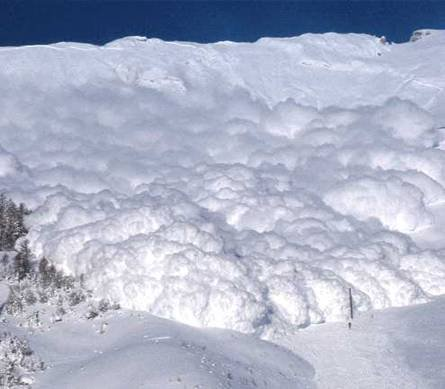
\includegraphics[width=\textwidth]{titlebackground.png}};\end{tikzpicture}}
%\usebackgroundtemplate{\tikz[overlay,remember picture]\node[opacity=0.4] at (current page.center){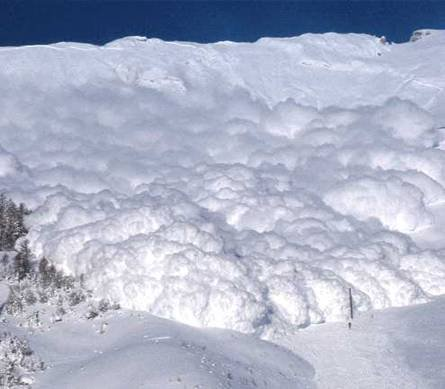
\includegraphics[width=3 in]{titlebackground.png}};}

\begin{frame}[plain]
\maketitle
\vspace{-3em}
\begin{columns}
        \column{0.25\textwidth}{
                
\includegraphics[width=0.94\textwidth]{logos/ncsu.png}
        }
        \column{0.50\textwidth}{}               
        \column{0.25\textwidth}{
                \begin{center}
                \includegraphics[width=0.94\textwidth]{logos/NSF_logo.png}
                {\tiny{ NSF DMR-0644743}}
                \end{center}
        }
\end{columns}
\end{frame} 
% RESTORE PRESENTATION STYLING
\setbeamertemplate{background}{}
\setbeamercolor{background canvas}{bg=white}

%%%%%%%%%%%%%%%%%%%%%%%%%%%%%
%%% end title page
%%%%%%%%%%%%%%%%%%%%%%%%




%%%%%%
% input section files

%\input{section1.tex} 
%\input{section2.tex} 
%\input{section3.tex} 


\begin{frame}
  \frametitle{Table of Contents}
  \tableofcontents
  Click TeX Refresh (F5) to update table of contents.
\end{frame}

\section{Videos}

%\ WORKS    
\begin{frame}
    \frametitle{Example 2}
    
    An example full frame video using the \textbf{basic syntax} is on this slide. This will play externally using default player.
    
    \vspace{20pt}
    
    \href{run:apollo17.avi}{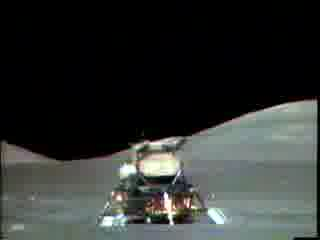
\includegraphics[height=0.7\textheight]{outputFrame_16.jpeg}}
\end{frame}

\begin{frame}
    \frametitle{Example 2: Test Graphics Path}
    
    An example of a single frame video using the graphics path.
    If this doesn't work, the next slide shouldn't work.
    
    \vspace{20pt}
    
    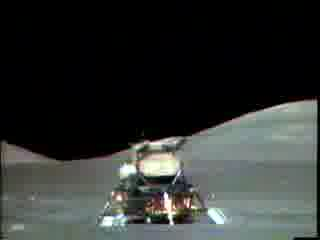
\includegraphics[height=0.7\textheight]{outputFrame_16.jpeg}
\end{frame}



\begin{frame}

\frametitle{Example using animate}
Here is an example using the animation package for playing within the pdf.
\begin{figure}
% here fps = 8, images are 1 through 42, show every image
\animategraphics[loop,width=.7\linewidth,every=1]{8}{outputFrame_}{1}{42}
\end{figure}
\end{frame}


% % DOES\ NOT\ WORK
% \begin{frame}
%     \frametitle{Example}
%     
%     An example full frame video using \textbf{commands from extrabeamercmds} is on the next slide. This does not work on Windows 10 or Ubuntu 15.10.
% 
% \fullFrameMovie[loop]{apollo17.avi}{apollo17.jpg}{\CopyrightText{Apollo 17, NASA}}
% \end{frame}
%     
% 
% 
% %\ DOES\ NOT\ WORK
% \begin{frame}
%     \frametitle{Example 3}
%     
%     An example full frame video using \textbf{commands from extrabeamercmds} is on the next slide. This does not work on Windows 10 or Ubuntu 15.10.
% 
% 
% % this assumes you have a .jpg named the same thing as your .avi
% \fullFrameMovieAvi[noloop]{apollo17}{\CopyrightText{Apollo 17, NASA}}
% \end{frame}
%     

\section{Citations}

\begin{frame}
\frametitle{Footnote Cite Demo}

%\noindent
\begin{itemize}
\item articles:

\citeintitle{einstein1905} versus \citejournal{einstein1905}. 
We can also add abbreviated footnote citations\autocite{einstein1905}
, which is good. We can cite it again and say \ctauthoryear{einstein1905} is an excellent paper. 
Remember to call ctfoot if you want the bibliography to print out at the bottom\ctfoot{einstein1905}

\citeintitle{yoon} versus \citejournal{yoon} 

\item books:

\citeintitle{salam} versus \citebooktitle{salam} 

\citeintitle{moraux} versus \citebooktitle{moraux} 

\citeintitle{pines} versus \citebooktitle{pines}
\end{itemize}
\end{frame}

\section{General Features}

\subsection{Outline}

\begin{frame}
  \frametitle{Presentation Outline}
  \framesubtitle{Using sectioning commands}

  You can use \texttt{\textbackslash section}
  and \texttt{\textbackslash subsection} commands
  to define outline of your presentation.

  These commands must be appeared between frames.
  Insert they manually in text source window. 

  To take correct outline under \TeX-Word click F5 key.

\end{frame}

\subsection{Overlays}

\begin{frame}
  \frametitle{Simple Overlays}
  \framesubtitle{Using pause command}

  The easiest way to create overlays is in using 
  the \texttt{\textbackslash pause} command.
  Like following ...

  \begin{itemize}
    \item This item is before \texttt{pause} (look source window)\pause
    \item If you don't see overlay read explanation below ...
  \end{itemize}

  Overlay expansion may be enabled/disabled 
  in dialog opened by `Insert/Document Properties' menu command.

  `\textit{Overlays Mode=\textbf{Handout}}' 
   -- disables overlay expansion.

  It is default setting of this template, 
  because this mode is convenient at
  first stage of developing slides.

  `\textit{Overlays Mode=\textbf{Beamer}}' 
   -- enables overlay expansion.

  It is useful at final editing 
  for handling overlays and for generating 
  final slides in form of PDF file.

\end{frame}

\subsection{Advanced Features}

\begin{frame}
  \frametitle{Advanced Overlays}
  \framesubtitle{Using more flexible overlay specifications}

  Beamer includes more ways for handling 
  overlays\dots
  \begin{itemize}
  \item using the \texttt{pause} command:
    \begin{itemize}
    \item
      First item.
      \pause
    \item    
      Second item.
    \end{itemize}
  \item
    using overlay specifications:
    \begin{itemize}
    \item<3->
      First item.
    \item<4->
      Second item.
    \end{itemize}
  \item
    using the general \texttt{uncover} command:
    \begin{itemize}
      \uncover<5->{\item
        First item.}
      \uncover<6->{\item
        Second item.}
    \end{itemize}
  \end{itemize}

  To learn more about Beamer package 
  read original documentation.

\end{frame}

\section{Main Talk}

\subsection{It is only beginning}

\begin{frame}
  \frametitle{Blank Frame}
  Body.
\end{frame}

\begin{frame}{A mind map}

\includegraphics[height=0.8\textheight]{mindmap.tikz}


\end{frame}

\section*{Conclusion}

\begin{frame}
  \frametitle{Conclusion}

  Clicking right mouse button 
  (press+release without intermediate mouse moving) 
  displays context menu
  which have two commands specific for beamer package: 

  \begin{itemize}
  \item
     \alert{Delete the Frame} -- removes current frame.
  \item
     \alert{Duplicate the Frame} -- easiest frame populating.
  \end{itemize}

  The button 
  at left edge of text 
  tool bar lets you insert blank slide in your presentation.

\end{frame}


\begin{frame}[allowframebreaks]
\frametitle{Bibliography}
%\topskip=2cm\advance\textheight by -2cm\enlargethispage{-1cm}
%\defbibheading{empty}{}
%{\Large Bibliography}
\printbibliography
\end{frame}


\end{document}
